\documentclass[review]{acmsiggraph}

\TOGonlineid{XXX}
%\title{A Polyfill Approach to Declarative Integration of Interactive 3D Graphics\\ into the World-Wide Web}
\title{Declarative Integration of Interactive 3D Graphics into the World-Wide Web:\\Principles, Current Approaches, and Research Agenda}
\author{Name Lastname\thanks{e-mail:name.lastname@someemail.com}\\Some Research Institution}
\pdfauthor{Name Lastname}

\keywords{Declarative 3D, HTML, DOM, Polyfill}

\begin{document}

\maketitle

\begin{abstract}
With the advent of WebGL, plugin-free hardware-accelerated interactive 3D graphics has finally arrived in all major desktop Web browsers.
WebGL is an imperative solution that is tied to the functionality of rasterization API. Consequently, its usage requires a deeper understanding of the rasterization pipeline. In contrast to this stands a declarative approach with an abstract description of the 3D scene. We strongly believe that such approach is more suitable for the integration of 3D into HTML5 and related technologies such as XML (that could be used for scene construction), DOM (could be used for scene manipulation), and CSS (could be used for styling), concepts known to the millions of existing Web developers and therefore crucial for the fast adoption of 3D on the Web.

As the participants of the \textit{Declarative 3D for the Web Architecture W3C Community Group}, we explore the options for new declarative ways of incorporating 3D graphics directly into HTML to enable its use on any Web page. In this paper we present Declarative 3D principles that guide the work of the group. We describe the current state of the fundamental to our initiative experimental X3DOM and XML3D frameworks. Finally we draw the agenda for the next development stage of the Declarative 3D for the Web.
\end{abstract}

\begin{CRcatlist}
  \CRcat{I.3.7}{Computer Graphics}{Three-Dimensional Graphics and Realism}{Virtual Reality}
  \CRcat{I.3.6}{Methodology and Techniques}{Standards}{Languages}
\end{CRcatlist}

\keywordlist
\copyrightspace

\section{Introduction}
The Web evolved from a text-based system to the current rich and interactive medium that supports images, 2D graphics, audio and video. These types of new media have made the Web experience richer, more attractive to users, etc, than ever before, and opened up possibilities for new types of applications and usage. The major media type that is still missing is 3D: synthetic, possibly photorealistic images in 3D with animation, as smoothly integrated in the everyday Web experience as images or video. Just as the appearance of images or video could open new application possibilities, access to the 3D on a Web site would make it possible to include realistic models of 3D objects (from models of buildings to representation of the human body or the sceneries for computer games). As of today, such applications require separate applications or the installation of browser plugins; however the goal would be to achieve the same smooth inclusion of 3D content in a Web page like we experience today with images or SVG based 2D graphics.

Although some of these goals could also be achieved by imperative means (e.g., through the usage of WebGL \cite{Khronos-WebGL}), developments of 3D models have a long tradition of using declarative approaches, which is also in line with some of the fundamental principles of Web development. It is therefore important to explore how the experiences accumulated in two different communities, namely the Web Development and Computer Graphics communities, can be capitalized upon to achieve the long term goal of using 3D on the Web the same way as we do with 2D graphics and video today.

\begin{figure}[ht]
  \centering
  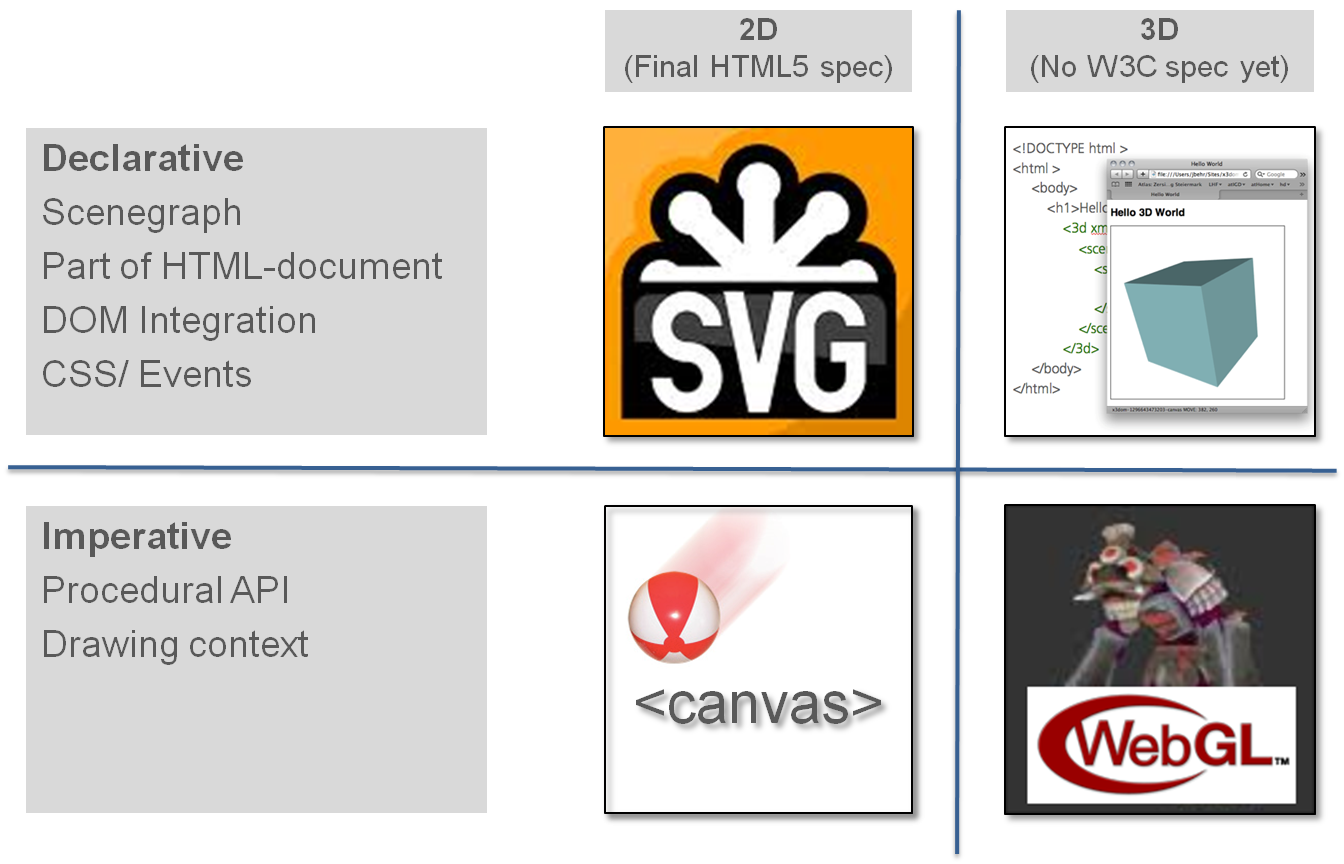
\includegraphics[width=\linewidth]{images/Declarative3d.png}
  \caption{The position of the Declarative 3D approach in the current Web graphics technology ecosystem.}
  \label{fig:DeclarativeVsImperative}
  %\vspace{-10px}
\end{figure}

It is arguable that the emerging support for an imperative 3D-API for the Web is useful but insufficient for broad acceptance and usage of 3D on the Web. A declarative approach that is tightly integrated with current web technologies and that offers qualified concepts is necessary to support a fast adoption and broad use of interactive 3D graphics by the millions of existing Web developers. The provided concepts must lift the hardware-oriented imperative application programming interfaces (APIs) to an expressive and more easily usable level. Therefore not the low-level data structures of existing hardware layers must be in the center of the design but high-level elements and items like 3D objects, transformations, material descriptions, and lights. Instead of teaching Web developers 3D graphics APIs, the goal is to bring 3D graphics to the point where its natural for Web developers to just make use of it. While this might not be possible for every possible use of a low-level API, we believe that it can cover the vast majority of use cases.

The \textit{Declarative 3D for the Web Architecture W3C Community Group} \cite{Dec3D-CG} has been formed to suggest and create methods to add interactive high-level declarative 3D objects to the HTML-DOM \cite{W3C-DOM}, so users can easily create, share and experience interactive 3D graphics. The core mission of this Community Group is to determine the requirements, options, and use cases for the declarative integration of interactive 3D graphics capabilities into the Web technology stack which will provide a foundation for future standardization.

This paper presents the current state and efforts of the Dec3D CG. In Section \ref{sec:Principles} we describe Declarative 3D principles: a number of key goals that guide the development of the DOM-based interactive 3D graphics within the Community Group.
In Section \ref{sec:Frameworks} we describe the current state of the fundamental to our initiative experimental systems: Fraunhofer's X3DOM \cite{Behr2009} and DFKI's XML3D \cite{Sons2010} declarative 3D Web publishing frameworks.
In Section \ref{sec:Agenda} we aim to shape the agenda and identify upcoming research issues for the next development stage of the Declarative 3D for the Web. Finally, in Section \ref{sec:Conclusions} we conclude our work.

\section{Declarative 3D Principles}
\label{sec:Principles}
The following goals and principles should guide the development:

\paragraph{Following the Established Principles of the Web}
Declarative 3D is being developed to significantly lower the barrier for authoring 3D content for Web sites. It aims to lower the barrier by duplicating the key features that enabled the growth of the early Web and its further spectacular success.

\begin{description}
  \item [Separation of structure from content] - Underlying the Web from its earliest days was the separation of structure from content. The concept of a paragraph specified by the $<$p$>$ tag was separate from the content in the paragraph. Declarative 3D is attempting to bring the same separation of structure from content to 3D graphics inside of web pages. The concepts such as definitions of 3D objects, transformations, materials, etc. should be implemented in a declarative 3D description as an extension to HTML5 using any existing or future extension mechanism.
  \item [Separation of content from style] - One of the principles of the current Web is also the separation of content and style, most notably through CSS. The successful integration of SVG with HTML was made much easier due to the fact that SVG was already following this principle.
      The aim of the CG is to extend the use of CSS for styling 3D graphics. One example can be the use of the latest CSS3 3D Transforms to allow to manipulate not only 2D but also 3D objects in 3D space.
  \item [Use of the Document Object Model] - The Document Object Model (DOM) is a platform- and language-neutral interface that allows programs and scripts to dynamically access and update the content, structure and style of Web documents \cite{W3C-DOM}. Declarative 3D should use DOM API to examine and modify elements on the 3D scene and their attributes by simply reading and setting their properties.
      As DOM provides access to user actions (e.g., pressing a key or clicking a mouse button), it should also be used as a main interface to interact with 3D content.
\end{description}

Moreover, the CG should reuse existing W3C techniques (specifically from HTML5 and SVG) as far as possible and propose extensions only where 3D specific features are necessary or where they provide significant benefits. Where new concepts are introduced their relation to and effects on existing Web standards should be analyzed, evaluated, and discussed with the respective W3C working groups.

\paragraph{3D Content Creation and Reuse}
While the creation of original 3D geometry and appearances still requires 3D specific know-how, the reuse, configuration, and manipulation of such content should be made similarly easy as for 2D Web content now. The solution should hide internal data structures and algorithms and provide users convenient ways to edit and manipulate such scenes.
A key success factor for Declarative 3D on the Web will be the ability to generate new or reuse existing content. This requires that suitable exporters and converters can be built. However, as 3D on the Web is supposed mainly as a delivery mechanism, it is not necessary to include the ability to semantically represent all but the important 3D features

\paragraph{Platform Independence}
The aim of the CG is to describe 3D content in a way that does rely neither on a specific render API such as OpenGL or DirectX nor on a specific rendering technique such as rasterization or ray tracing only. The technology investigated should allow for content to be portable across user agents, rendering techniques, and hardware platforms, while taking advantage of available features wherever possible. The results of rendering content under such different environments should be highly predictable.

\paragraph{Efficiency and Scalability}
Interactive 3D graphics operates in real-time, which enables new forms of interactivity on the Web but also adds significant new requirements on user agents.  A key requirement for the selected technology therefore is the possibility to implement it efficiently. Since 3D scenes can sometimes become large, any solution should target scalability in the sense that 3D content should run across different platforms (from mobile devices to high-end graphics hardware) with predictable performance. Mechanisms should be in place to handle cases where the performance provided by a user agent on some platform is not sufficient, e.g. by allowing for switching to different content (e.g. lower LOD) or provide alternate methods of delivering the content (e.g. server-based rendering delivered via streaming video).

\paragraph{Security \& Digital Rights Management}
Secure delivery of Web content is a general problem and not specific to 3D data. However, the economic value of 3D data might make the problem more acute. Any proposed solution should therefore be based on a general approach to secure Web content. The CG should, however, collect use cases, extract requirements and examine how far existing methods and standards can be transferred to the proposed architecture. It is already demonstrated that application of XML Encryption and Signature is needed for document fragments as well as full documents, since high-fidelity or sensitive portions of 3D models often need special protections.

\paragraph{Accessibility \& Usability}
A large body of work has shown that accessibility improvements serve all users, not just people with disabilities.  A curious aspect of many 3D graphics approaches is that user navigation is implemented inconsistently.  Therefore, users familiar with one approach are impeded when navigating or interacting with other 3D scenes and models.  Examination of relevant Web Accessibility Initiatives (WAI) principles might provide significant benefit.  Conversely, use of declarative 3D graphics models might provide major benefits when describing the accessibility features and constraints of real-world objects and locations.  Declarative 3D goals and potential solutions may achieve significant benefits if they are harmonizable with WAI imperatives.

\newpage

\section{Declarative 3D Experimental Frameworks}
\label{sec:Frameworks}
As we have already mentioned, our Community Group has been formed to determine the requirements, options, and use cases for the declarative integration of interactive 3D graphics capabilities into the Web technology stack which will provide a foundation for future standardization.
While the standardization is our goal, we still need platforms allowing for the experimentation and for the assessment of our design decisions. We also need to reach out to Web developers who could provide us with valuable feedback as early as possible.

In the following we briefly introduce two experimental open-source frameworks that support the ongoing discussion in the computer graphics and Web communities how an integration of HTML and Declarative 3D content could look like. This discussion is followed by the presentation of the \textit{polyfill} approach for the further X3DOM \& XML3D development activities.

\subsection{X3DOM \& XML3D}
Introduction to this section: Fraunhofer's X3DOM \cite{Behr2009} is an open-source framework that allows including X3D \cite{Web3D-X3D} elements as part of any HTML DOM tree... DFKI's XML3D \cite{Sons2010} is a similar approach...

In the second paragraph, I believe we should write something about the main similarities and differences of the frameworks (not going into details but more from philosophical point of view).

In the last paragraph of this section, we can write about the efforts to consolidate approaches and/or how the competing two frameworks influence one another for the common benefit...? This should be followed by the some link to the next section (polyfill).

\newpage

\subsection{Polyfill Approach}
Recently, the CG proposed to measure a level of integration for 3D graphics in terms of W3C technologies (DOM, CSS etc) \cite{Dec3D-LevelsOfIntegration}. The proposal aims to explain existing and possible integration levels and finally to identify an integration level the CG is aiming for.

It quickly became clear that a higher level of integration requires additional APIs in user agents. After discussions with browser vendors (namely Firefox and Chrome), who made it clear that integration of the desired extensions natively into their frameworks is not currently their priority, we decided to consider a polyfill approach for the further development activities of the Community Group.

A \textit{polyfill} is downloadable piece of code, which provides facilities that are not built-in to a Web browser \cite{Sharp2010}. For example, many features of HTML5 are not supported by versions of Internet Explorer older than version 8 or 9, but can be used by web pages if those pages install a polyfill. Polyfills can also be used to add entirely new functionality to browsers.

Polyfill based approaches allow the Declarative 3D Community Group to derive hard requirements for related and utilized W3C standards and UA APIs immediately. This leads to a much more evolving concepts and solutions in contrast to an overall declarative 3D specification.

\begin{figure}[ht]
  \centering
  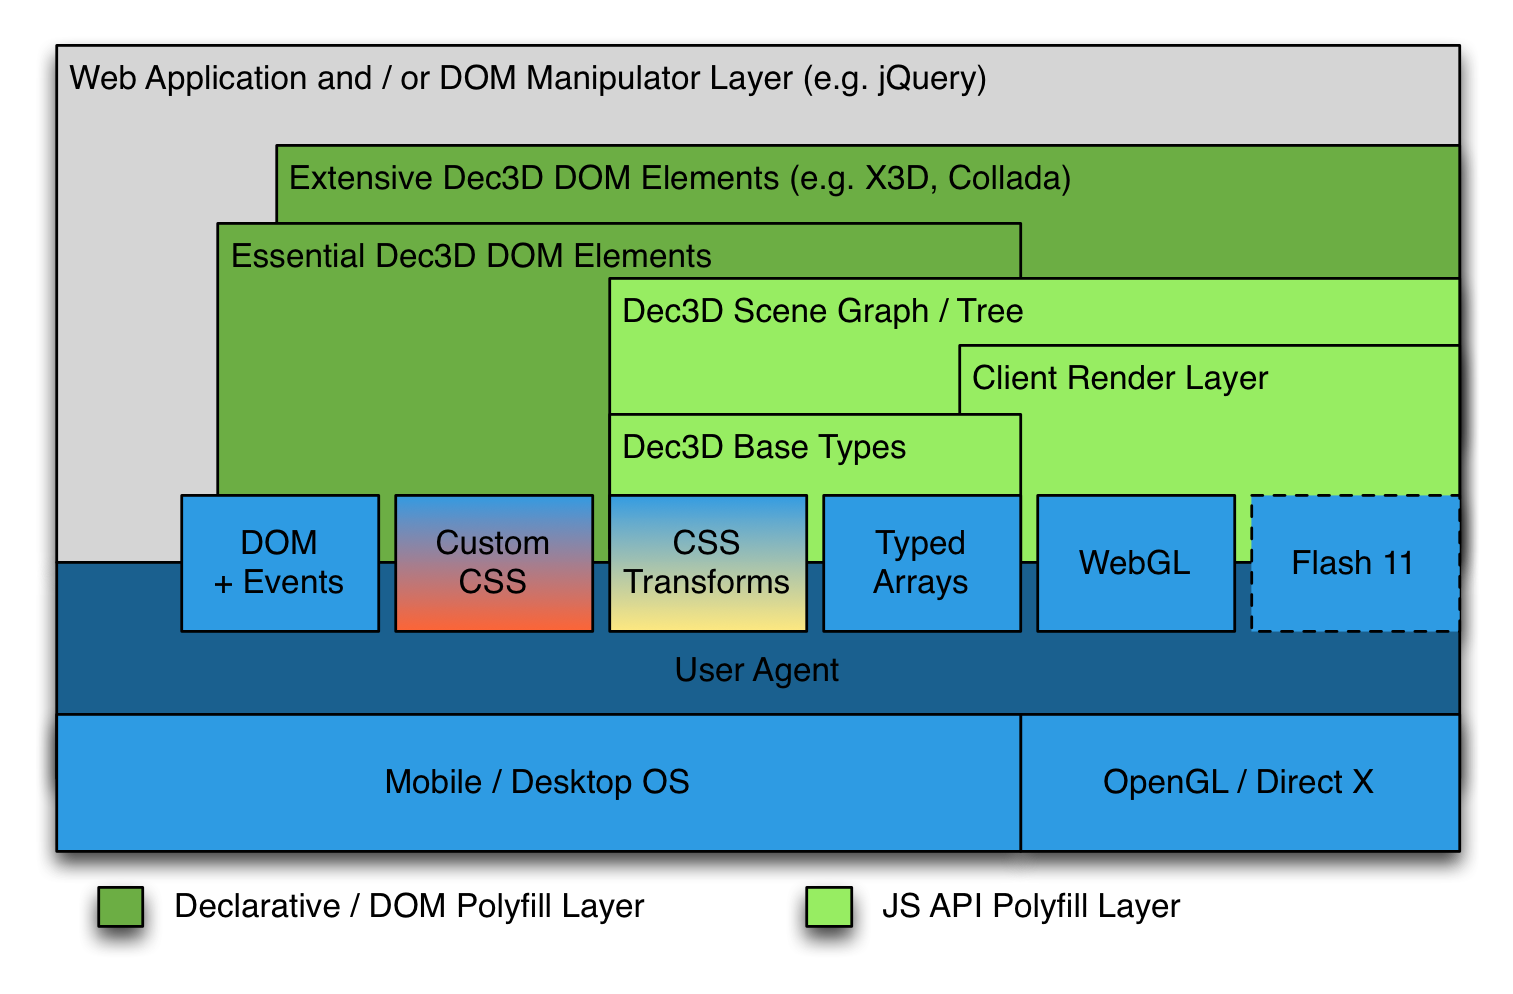
\includegraphics[width=\linewidth]{images/Dec3D-Architecture.png}
  \caption{Declarative 3D polyfill runtime architecture.}
\end{figure}

\begin{figure*}[ht]
  \centering
  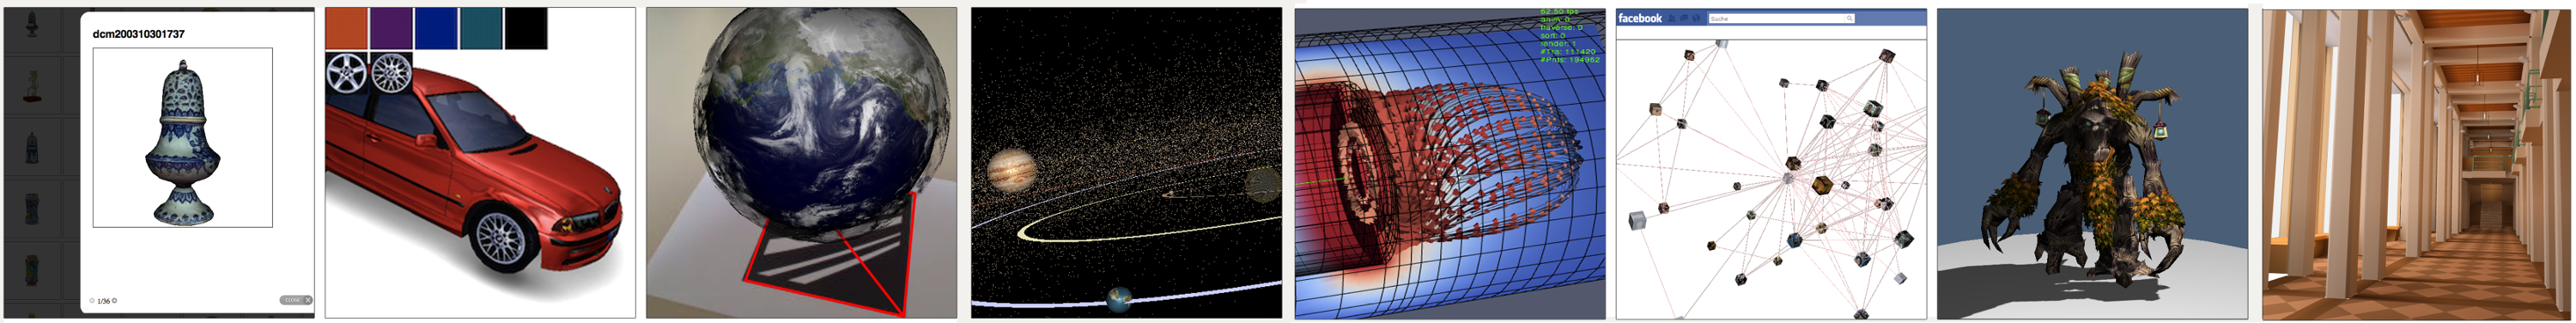
\includegraphics[width=\linewidth]{images/Demos.png}
  \caption{ToDo: Some latest examples of X3DOM and XML3D based Web applications.}
  \vspace{-7px}
\end{figure*}

To sum up, the X3DOM and XML3D experimental declarative 3D Web publishing frameworks were designed to explore different options for adding interactive 3D graphics to HTML. We want to stress that the whole integration model is still evolving and it is open for discussion.

\newpage

\section{Declarative 3D Agenda}
\label{sec:Agenda}
During the 1st International Workshop on Declarative 3D for the Web Architecture (Dec3D2012) \cite{Dec3D2012} as well as during more informal group meetings at Web3D in 2011, 2012 and SIGGRAPH in 2011, 2012, the members and supporters of the Declarative 3D W3C Community Group agreed that what is needed to make the effort successful and for the W3C to adopt/develop a declarative 3D standard is:

\paragraph{Encourage Participation}
All relevant stakeholders, e.g. developers, designers, researchers, 3D artists, industry professionals, representatives of standards organizations, accessibility experts, and user-agent implementers, are encouraged to participate in the Declarative 3D Community Group. Participants must be willing to actively develop and donate materials towards the group's deliverables, as well as attend the group's teleconferences and face-to-face meetings.

\paragraph{Clear Definition of Use Cases \& Requirements}
The Community Group needs to agree on a collection of use cases, where embedding 3D data in HTML using declarative approach provides significant benefit. Each use case should explore how publishers and consumers benefit from Dec3D. From these use cases, the Community Group needs to derive and prioritize the different required dimensions for the Declarative 3D technical specification (see \cite{JankowskiDec3D2012,LeFeuvreDec3D2012}).

\paragraph{Clear Technical Specification}
The next step of the CG should be the creation of the clear, detailed and extensible technical specification of the implementation concepts and features necessary to cover the majority of useful requirements (but not necessarily all of them). Measurable properties should be defined to quantitatively or qualitatively evaluate the quality of the solution, document the pros and cons of each solution based on these measurements, demonstrate that, based on the above analysis, there is a good chance of success in creating a W3C standard for Declarative 3D for the Web.

\paragraph{Outreach \& Killer App}
The CG needs to continue its outreach activities through the high quality demonstrations of the Declarative 3D philosophy using the experimental X3DOM and XML3D frameworks. It should also consider focusing on one killer application of Declarative 3D, an application so necessary or desirable that it proves the core value of the Declarative approach and that could substantially increase the visibility of the CG's efforts.

\paragraph{W3C Working Group Proposal}
Finally, the Community Group should deliver a report documenting its progress, any conclusions it arrived at with respect to standardization of \textit{Declarative 3D for the Web} and, if reaching a positive conclusion, recommending a standardization approach as a basis for a future W3C working group on the same topic.

\newpage

\section{Conclusions}
\label{sec:Conclusions}
While WebGL 3D imperative graphics API in the Web context is getting more and more traction, we are still missing an easy way to add interactive high-level declarative 3D objects to the HTML to allow anyone to easily create, share, and experience interactive 3D graphics – with possibly wide ranging effects similar to those caused by the broad availability of video on the Web.

The goal of the Declarative 3D CG is to evaluate the options for a successful standardization of a declarative approach to interactive 3D graphics as part of HTML documents. The goal is to collect suitable use cases, derive requirements from them, and then find the essential set of features and concepts that enables broad uptake by authors and users of interactive 3D on the Web.
We are absolutely aware that our goal is ambitious and it will take some time to implement these features. Therefore, we call for more participation from the 3D Web community that we believe is crucial to achieve our common and ultimate goal: 3D for everyone and everywhere.


%\section*{Acknowledgements}
\bibliographystyle{acmsiggraph}
\bibliography{bibliography}
\end{document}
